\chapter{Data set}
\label{ch:dataset}
 
%
% Section: 4 - Intro
%

Training and evaluation of automatic information extraction approaches requires availability of reliable ground truth data of sufficient size. Following a growth of interest for extraction of information about software tools from scientific publications labeled data sets with limited scope such as BioNerDs, SoftCite, SoSciSoSci have came into existence. More recently, \ac{SoMeSci} data set, a more comprehensive corpus that covers a wide range of information about software tools has also been introduced \citep{schindler2021somesci}.  \\

This section describes the data set used in this project – \ac{SoMeSci},  the extension process with software usage purpose annotations, issues observed during annotation, pre-processing of the data-set, analysis results of the data and transformation to a suitable format for training purpose.  


\section{SoMeSci data set}
\label{sec:dataset:SoMeSci}

\ac{SoMeSci} data set contains high quality, hand annotated articles collated from  \ac{PMC}. The articles and annotations included in the data set are summarized below.  

\subsection{ SoMeSci Articles }
\label{subsec:dataset:SoMeSci:Articles}

The corpus is composed of four group of files, namely\emph{PLoS methods, PLoS sentences, PubMed full text} and \emph{Creation sentences}. Facts about the articles in the \ac{SoMeSci} corpus is summarized in the table 4.1 below.

\begin{table}
	\caption{Article composition of  \ac{SoMeSci} dataset.}
	\begin{tabularx}{\textwidth}
		{|>{\setlength\hsize{.6\hsize}\setlength\linewidth{\hsize}}X|>{\setlength\hsize{1.4\hsize}\setlength\linewidth{\hsize}}X|}
		
		\hline
		SoMeSci article & Description  \\
		\hline
		1. PLoS Methods   &
		- 480 articles from PLoS journal that contain only methods sections\\
		\hline
		2. PubMed full text   &
		- 100 randomly selected full-articles from PMC Open Access\\
		\hline
		3. PLoS sentences  &
		- 677 files extracted from PLoS articles which contain sentences that has software names mentioned in them.  \\
		\hline
		4. Creation sentences  &
		- 110 files that contain sentences indicating creation of a software  files out of which 50 are extracted from PMC OA, where as the rest 60 are from PLoS.  \\
		\hline
		
		\emph{Total} &
		- 1367 files  \\
		\hline

	\end{tabularx}
\end{table}

\subsection{SoMeSci Annotations  }
\label{subsec:dataset:SoMeSci:Annotations }

SoMeSci corpus has three main types of annotations that correspond to a type of information related with software tools. These annotations indicate the type of software, type of mention and additional information about the software as summarized on the table below:


\begin{table}
	\caption{Annotation composition of \ac{SoMeSci} dataset before its extension with software usage purpose labels.}
	\begin{tabularx}{\textwidth}
		{|>{\setlength\hsize{.6\hsize}\setlength\linewidth{\hsize}}X|>{\setlength\hsize{1.4\hsize}\setlength\linewidth{\hsize}}X|}
		
		\hline
		Type of Annotation & Description  \\
		\hline
		4 software-types   &
		- Application, Plugin, Operating System and Programming Environment\\
		\hline
		4 mention types  &
		- Mention, Usage, Creation, and Deposition\\
		\hline
		9 additional info.  &
		- Developer, Version, URL, Extension, Release, License, Abbreviation, \& Alternative name.\\
		\hline
		
	\end{tabularx}
\end{table}

\section{Annotation tool}
\label{sec:dataset:tool}
The data set has been annotated using BRAT rapid annotation tool \href{https://scicrunch.org/resolver/SCR_008769}{RRID:SCR\_008769}, v.1.3 , in a Linux 20.4 environment. The annotation tool has been run in a local machine as a CGI application using a browser. 

\begin{figure}[htbp]
	\centering
	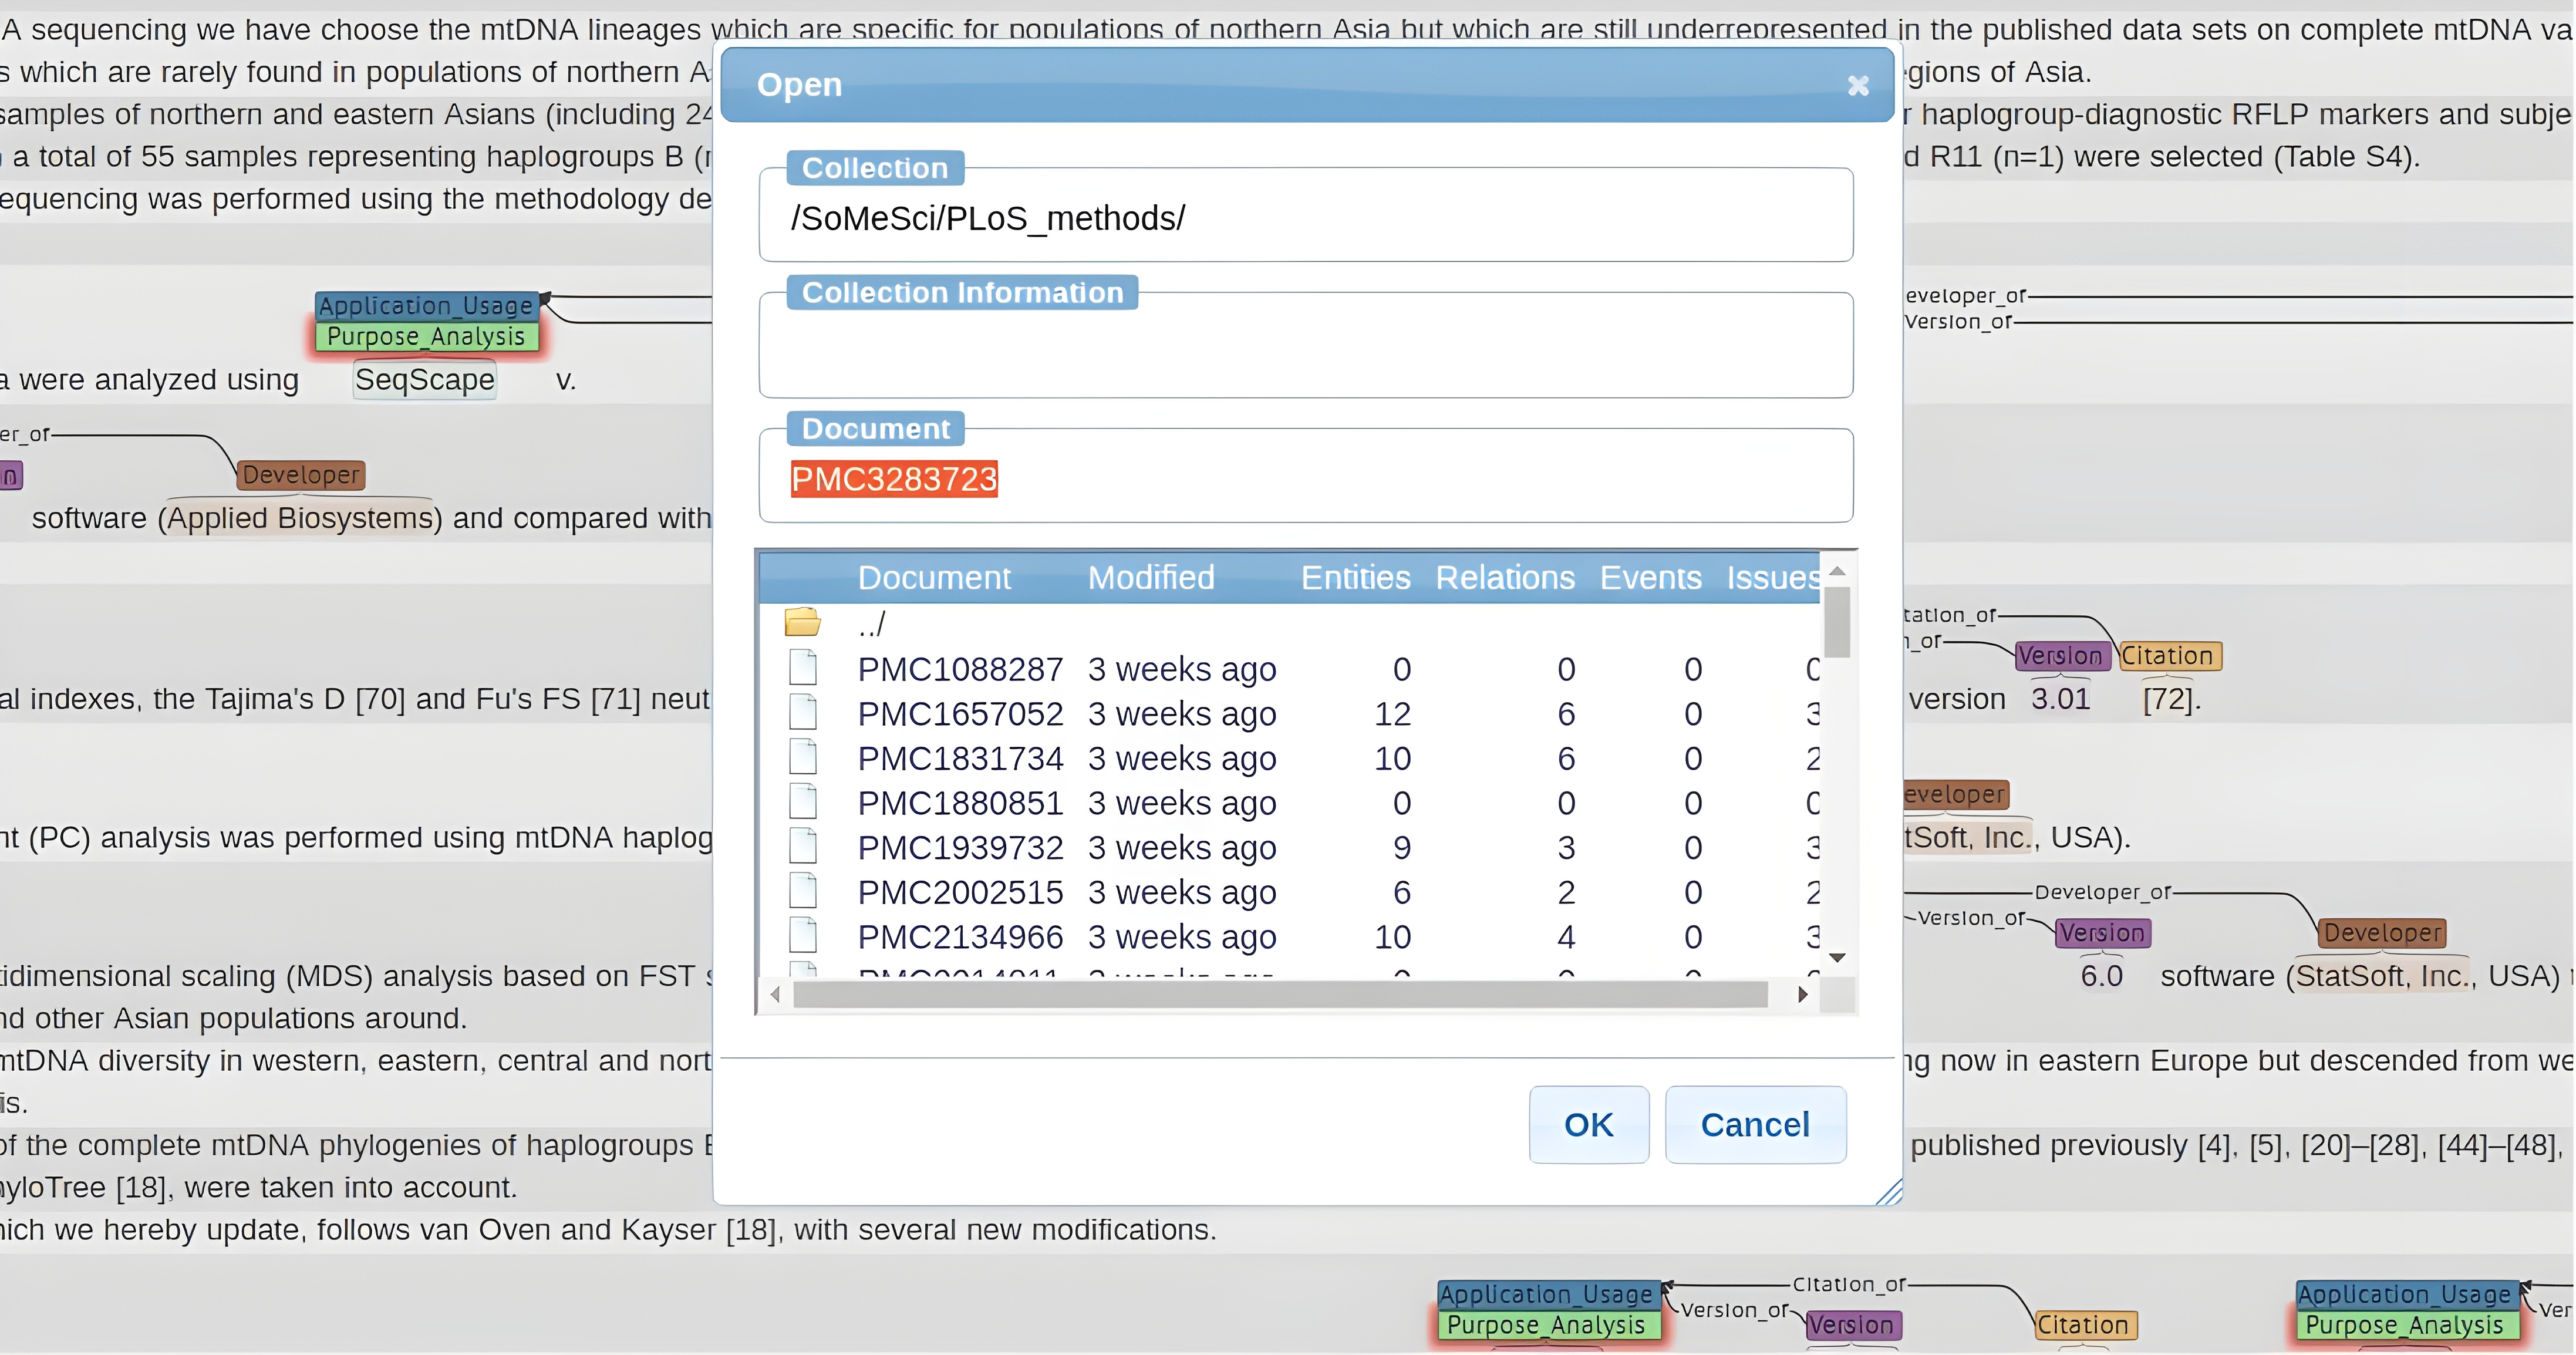
\includegraphics[width=.75\textwidth]{4.graphics/figures/ch_4/BRAT_tool}
	\caption{BRAT annotation tool}
	\label{fig:chapter04:setup}
\end{figure}

\subsection{Annotation of SoMeSci with software purpose labels}
\label{subsec:dataset:tool:Annotationprocess}

\ac{SoMeSci} corpus has been extended with annotations of eight classes of purpose of software usage labels identified in the earlier section. Since using software for a particular purpose only refers to the usage of a software, only usage labels has been further labelled with software purpose. The figures below show \ac{SoMeSci} data set before and after software purpose annotations. \\

\begin{figure}[htbp]
	\centering
	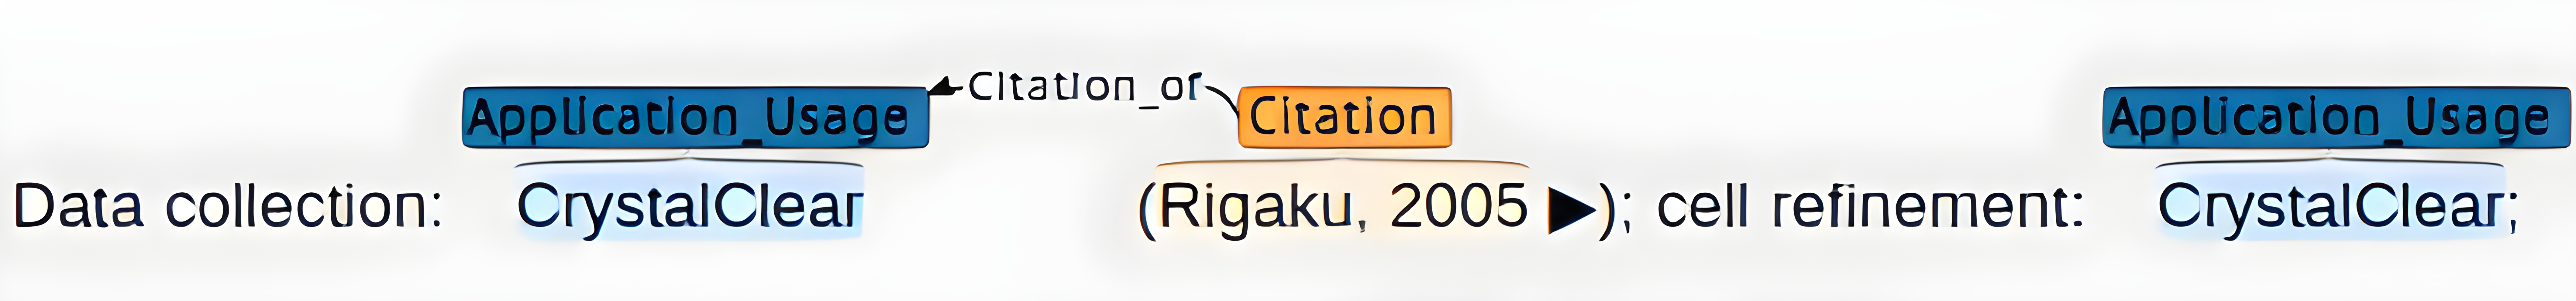
\includegraphics[width=.99\textwidth]{4.graphics/figures/ch_4/before_ann_hd_PMC3120364_FULLTEX_HD}
	\caption{Original annotations in \ac{SoMeSci} dataset before extension with software usage purpose annotations }
	\label{fig:chapter04:setup}
\end{figure}

\begin{figure}[htbp]
	\centering
	
\includegraphics[width=.99\textwidth]{4.graphics/figures/ch_4/after_ann_hd}
	\caption{\ac{SoMeSci} annotations after extension with software usage purpose labels}
	\label{fig:chapter04:setup}
\end{figure}


\subsection{Assumptions in the annotation}
\label{subsec:dataset:tool:Assumptions}

For the sake of simplicity, certain types of software usages have been assigned the same class of software purpose annotation. For example, modeling might refer to graphical modeling of an object using \ac{CAD} software or it might also refer to mathematical representation of a given problem.  All such variants of modeling tasks have been assigned “modeling” as a label without differentiating specific variants. 



\subsection{Challenges during Annotation }
\label{subsec:dataset:tool:Challenges}
Annotations has been carried out in a such way by deciding on each context which software purpose annotation is more important or based on the general goal of the software usage. For example, FlexArray software on the figure below, has been annotated with software purpose analysis even though the same software was used for visualization purpose as well. This is because on this context analysis is more important than visualization and essentially visualization could also be interpreted as one kind of analysis. In addition, specific definition of each of software usage purposes has been also taken into account. \\

\begin{figure}[htbp]
	\centering
	\includegraphics[width=.99\textwidth]{4.graphics/figures/ch_4/Ann_confusion_HD}
	\caption{Label importance}
	\label{fig:chapter04:setup}
\end{figure}

However, annotation of software usage statements was not often straightforward. This is because, in some instances, purpose of software usage appears to be ambiguous. For example a software used for counting or quantification can be assigned a software purpose label of  data collection but it is also possible to treat those tasks like analysis. Therefore such cases annotation of purpose label might become subjective, might affect the Inter-rater-reliability agreements and the  over all annotation quality.\\

The other challenge of annotation was difficulty arising from limited domain knowledge. 

\section{Data Pre-processing}
\label{sec:dataset:preprocessing}
Pre-processing of the data set has been carried out to ensure the integrity of our data set before using it in the classifier. The data pre-processing tasks handled annotation errors, merging annotations , transforming and splitting of data set. 

\subsection{Handling missing annotations and annotation errors }
\label{subsec:dataset:preprocessing:handlingerrors}

As described in the above table, the four types of software mentions in the SoMeSci are mention, usage, creation and deposition. The main goal of annotating the data set was to assign corresponding purpose of software usage label to each instance of software usage but not for mention, creation and deposition. However, due to an error there were some instances of software mention that has been annotated with software purpose. In addition to this, there were also some instances of usage, that has not been annotated and intentionally skipped because of the purpose of software usage did not seem to be clear. \\

Therefore, all instances of wrong or missing annotations have been identified automatically to ensure the integrity of training data set.The python code for automatic identification of annotation errors has been listed under \emph{Appendix B}.

\subsection{Merging annotations}
\label{subsec:dataset:preprocessing:Merging}

After handing all annotation errors and missing labels, annotations of software usage has been merged with annotations of software purpose. Merging of the annotations solves two problems. \\

First it will fix annotation error message that is displayed on the BRAT tool. The error message is displayed because more than one annotation per a token is not supported by the annotation tool. \\

The other reason for merging annotations is to take advantage of legacy code, ariclenizer, which will transform data from BRAT too in a stand-off format  into IOB format which is desirable for training purpose. The python code for merging annotations has been listed on the \emph{Appendix C}.

\begin{figure}[htbp]
	\centering
	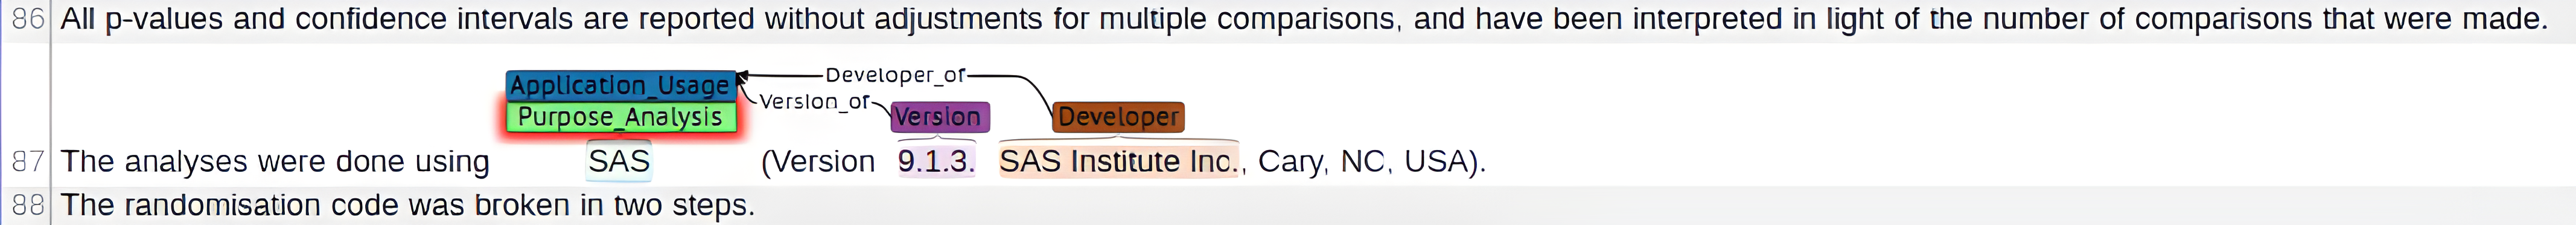
\includegraphics[width=.95\textwidth]{4.graphics/figures/ch_4/2002515_plm_unm_HD}
	\caption{Software usage annotations before merging with software purpose  annotation.}
	
	\label{fig:chapter04:setup}
\end{figure}

\begin{figure}[htbp]
	\centering
	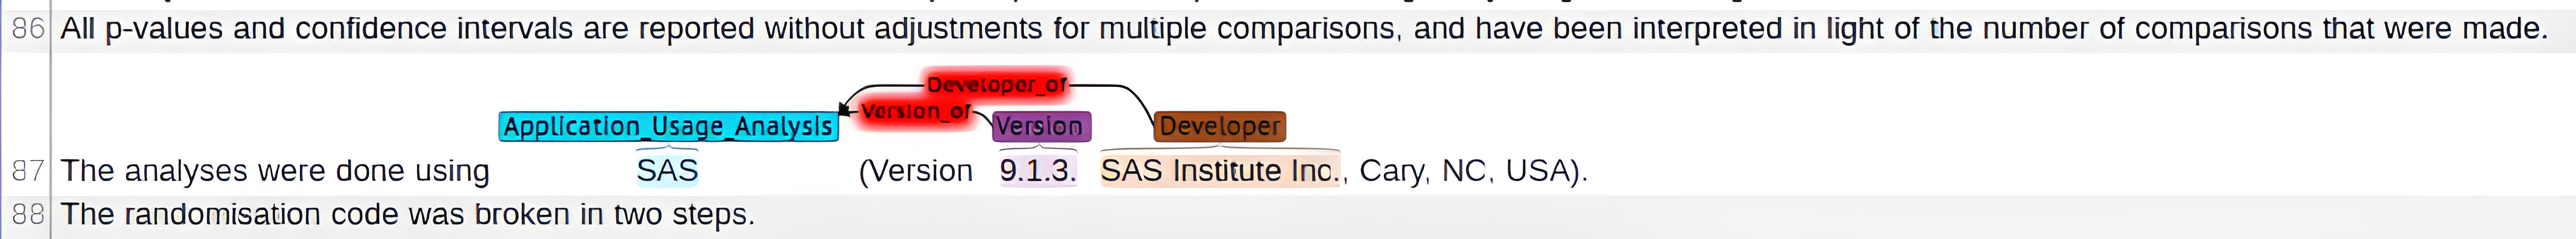
\includegraphics[width=.95\textwidth]{4.graphics/figures/ch_4/2002515_plm_HD}
	\caption{Software usage annotations after merging with software purpose  annotation.}
	\label{fig:chapter04:setup}
\end{figure}


\subsection{Transformation to IOB format}
\label{subsec:dataset:preprocessing:Transformation}
After merging software usage and purpose labels, transformation of data into IOB format has been carried out using articlenizer (link to articlenizer). Picture below shows the data format before and after transformation. \\

\begin{figure}[h]
	
	\myfloatalign
	
	\subfloat{
		\label{fig:chapter03:subfloat:grafik1}
		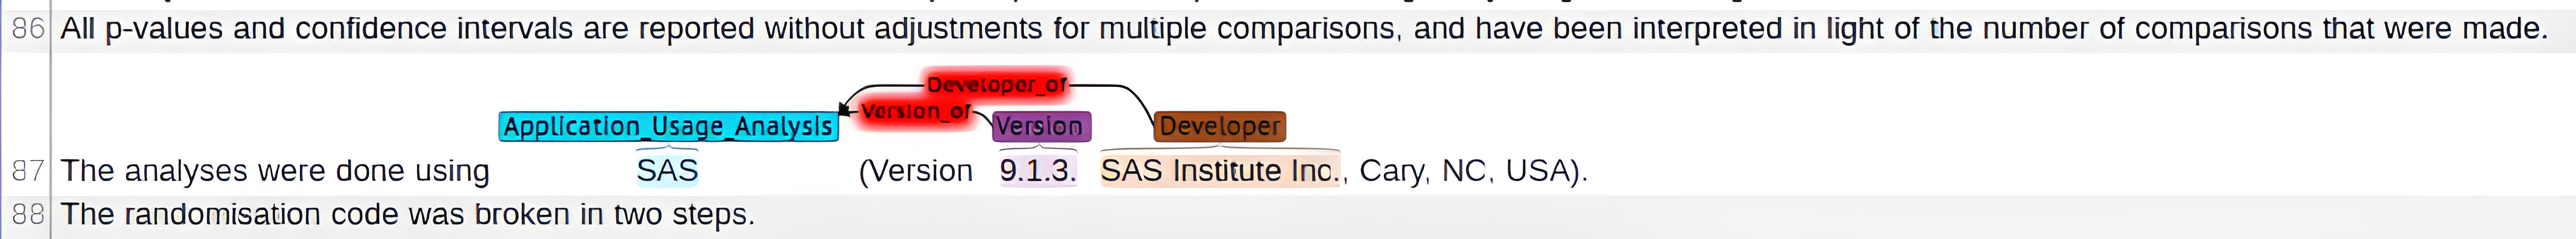
\includegraphics[width=.98\linewidth]{4.graphics/figures/ch_4/2002515_plm_HD}
	} \\
	\subfloat{
		\label{fig:chapter03:subfloat:grafik4}
		
\includegraphics[width=.98\linewidth]{4.graphics/figures/ch_4/BIo_2002515_plosmet_HD}
	}\\
	\caption[Subfloat - Figure]{Merged software usage and purpose annotation \& its corresponding BIO representation.}
\end{figure}

\subsection{Data Splitting}
\label{subsec:dataset:preprocessing:Splitting}
After the data has been transformed into the IOB format, it has been further split into training, development and test set in 60:20:20 ratio.


\section{Analysis of Annotated Data}
\label{sec:dataset:Analysis}

Analysis of cleaned SoMeSci data set has been carried out to find a deeper insight about the training data. 

\subsection{Co-reference resolution of software entities }
\label{subsec:dataset:Analysis:resolution}

The base line for the analysis of the data set was to carry out disambiguation of software names. This was particularly important because there is large degree of variation in software names. Using list of software name with corresponding URL, software mention instances have been disambiguated from each other and all software name variations that refer to the same entity have been given the same name. \\

Figure below shows name variations for MATLAB software, in which all instances resolve to the same URL i.e. entities referring to the same software. All variations of names has been replaced by the first “Matlab” in this case.

\begin{figure}[htbp]
	\centering
	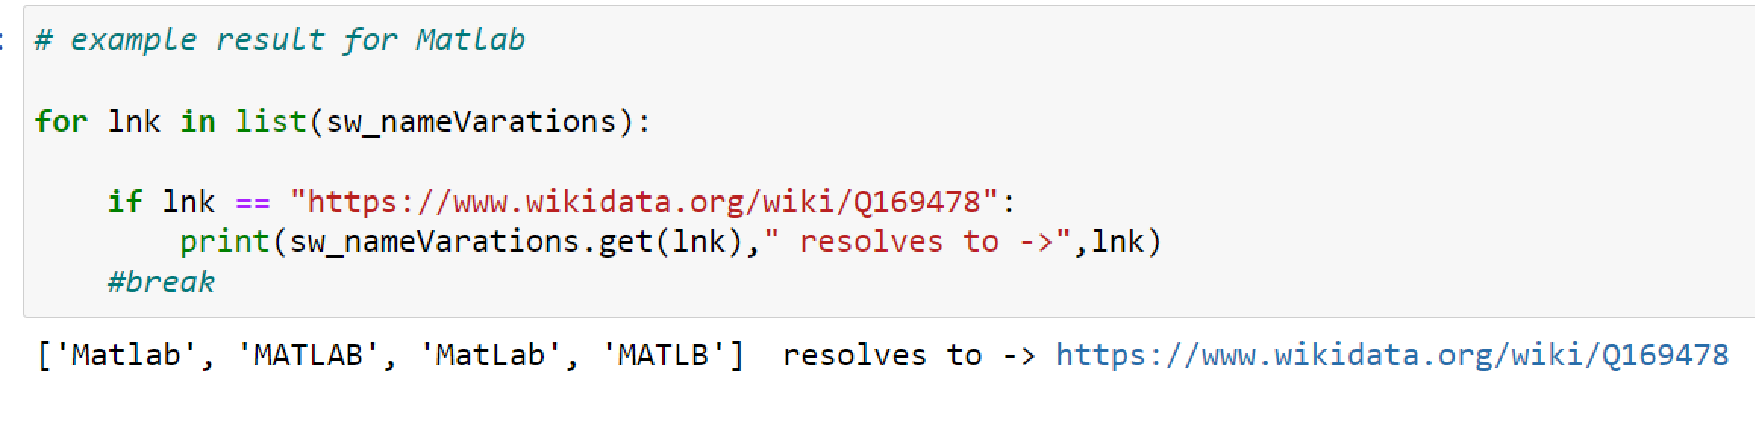
\includegraphics[width=1\textwidth]{4.graphics/figures/ch_4/pdf/Corefresolution}
	\caption{Example of Co-reference resolution for Matlab software. All name variations have been given the same name.}
	\label{fig:chapter04:setup}
\end{figure}


\subsection{Analysis results }
\label{subsec:dataset:Analysis:results}

According to the analysis results, the top 3 software by number of software name mention count through out the list of articles in PubMed and PLoS data set are: PASW, GNU-R and STATA.  

\begin{figure}[htbp]
	\centering
	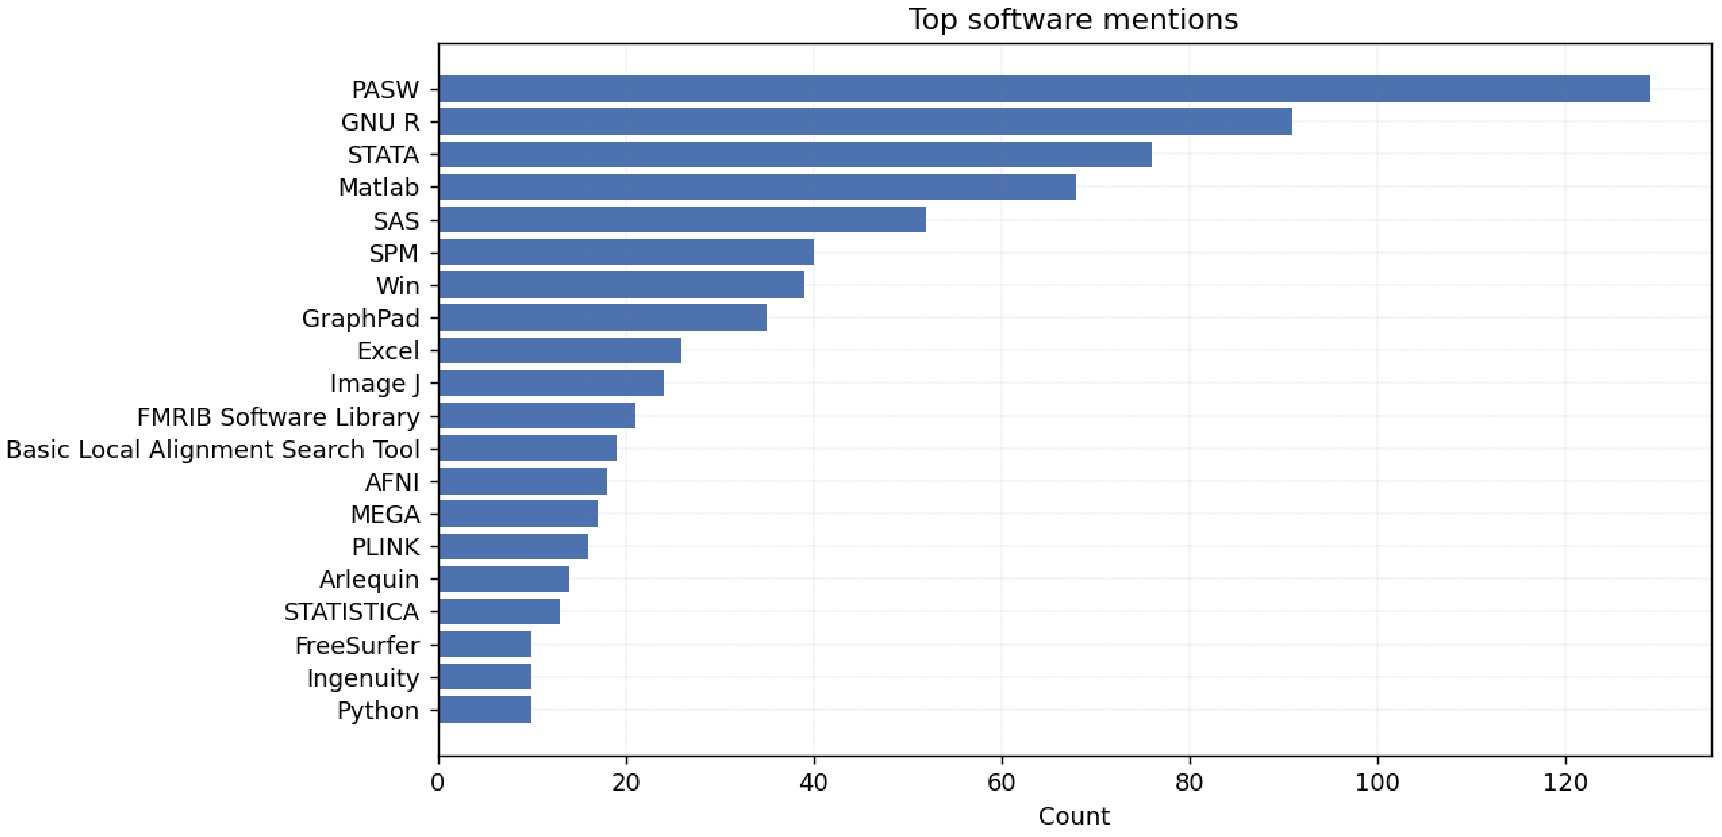
\includegraphics[width=1\textwidth]{4.graphics/figures/ch_4/analysisresults/1.Top software mentions}
	\caption{Top software mentions}
	\label{fig:chapter03:setup}
\end{figure}

Data set analysis result from the perspective of purpose of software usage indicates that, the most common purpose of software usage are: Analysis, Data pre-processing, Data collection and modelling where as the least common are simulation and stimulation. The result is shown on figure 4.10 below. \\

The other insight form from  the software-type perspective, is that the most commonly used type of software in the research articles in the data set is Application software as depicted on figure 4.11. \\

\begin{figure}[h]
	\myfloatalign
	\subfloat[software purpose]{
		\label{fig:chapter03:subfloat:grafik1}
		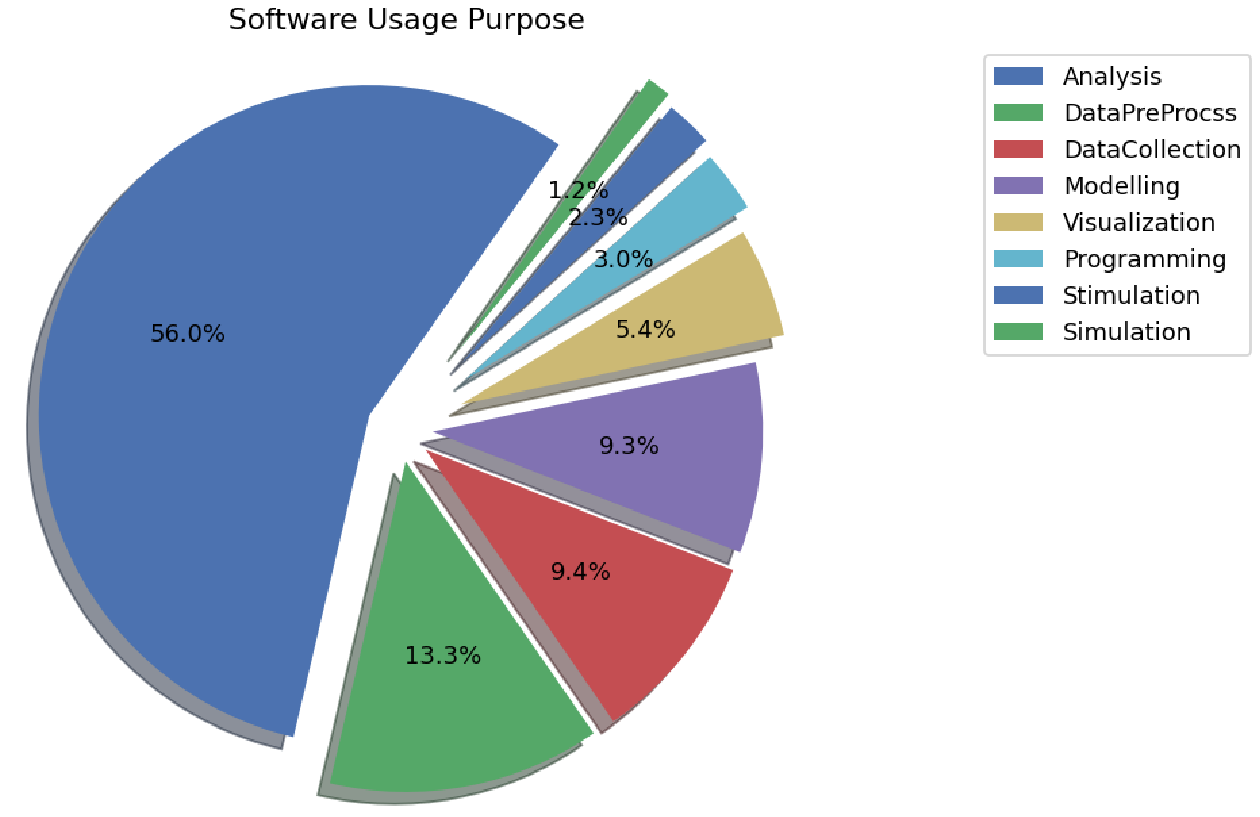
\includegraphics[width=.46\linewidth]{4.graphics/figures/ch_4/analysisresults/2.Software Usage Purpose pie}
	} \quad
	\subfloat[Types of software] {
		\label{fig:chapter03:subfloat:grafik2}
		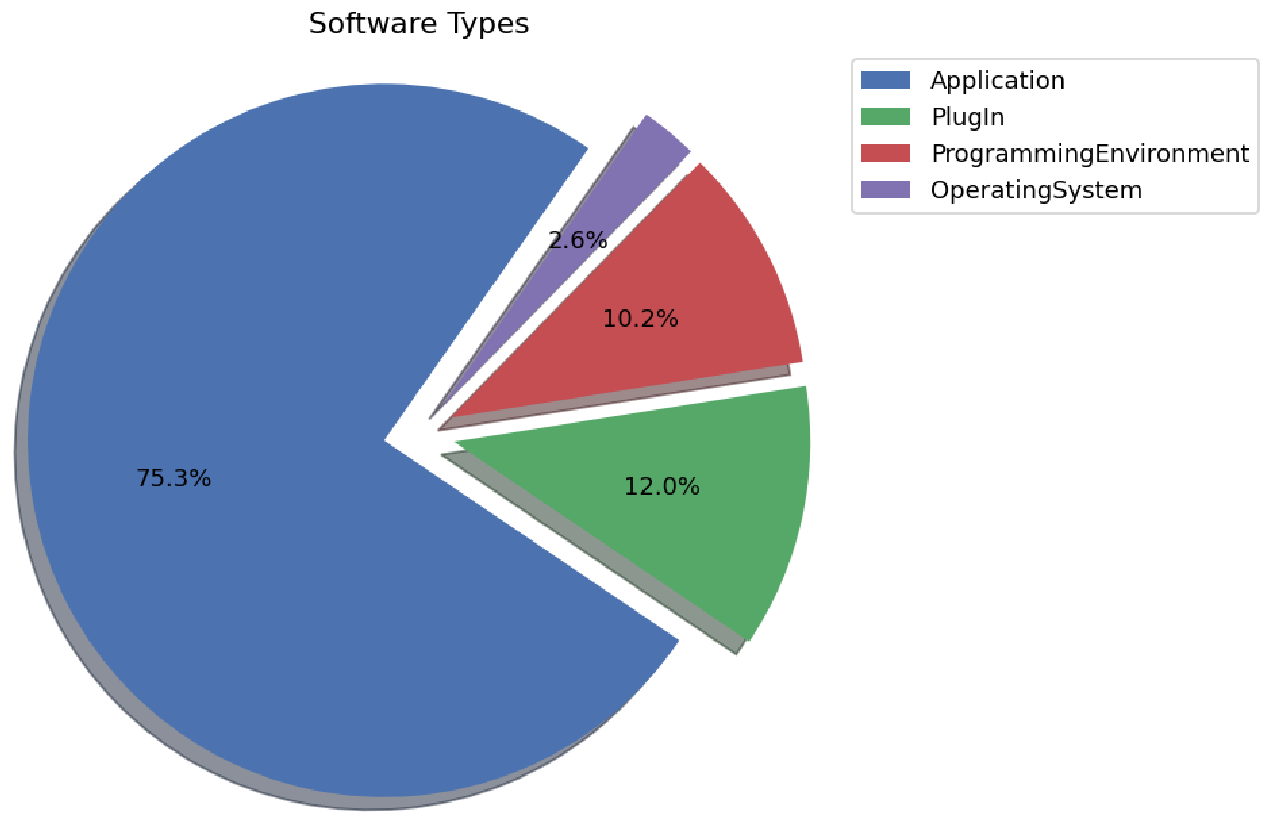
\includegraphics[width=.46\linewidth]{4.graphics/figures/ch_4/analysisresults/4.Software Types pie}
	} \\
	\caption[Subfloat - Figure]{}
	
\end{figure}


When it comes to share of each purpose of software usage among the 4 types of software, the pattern once again clearly indicates most of the time a software has been used for the purpose of analysis and data collection in all of the four software types. \\

\begin{figure}[htbp]
	\centering
	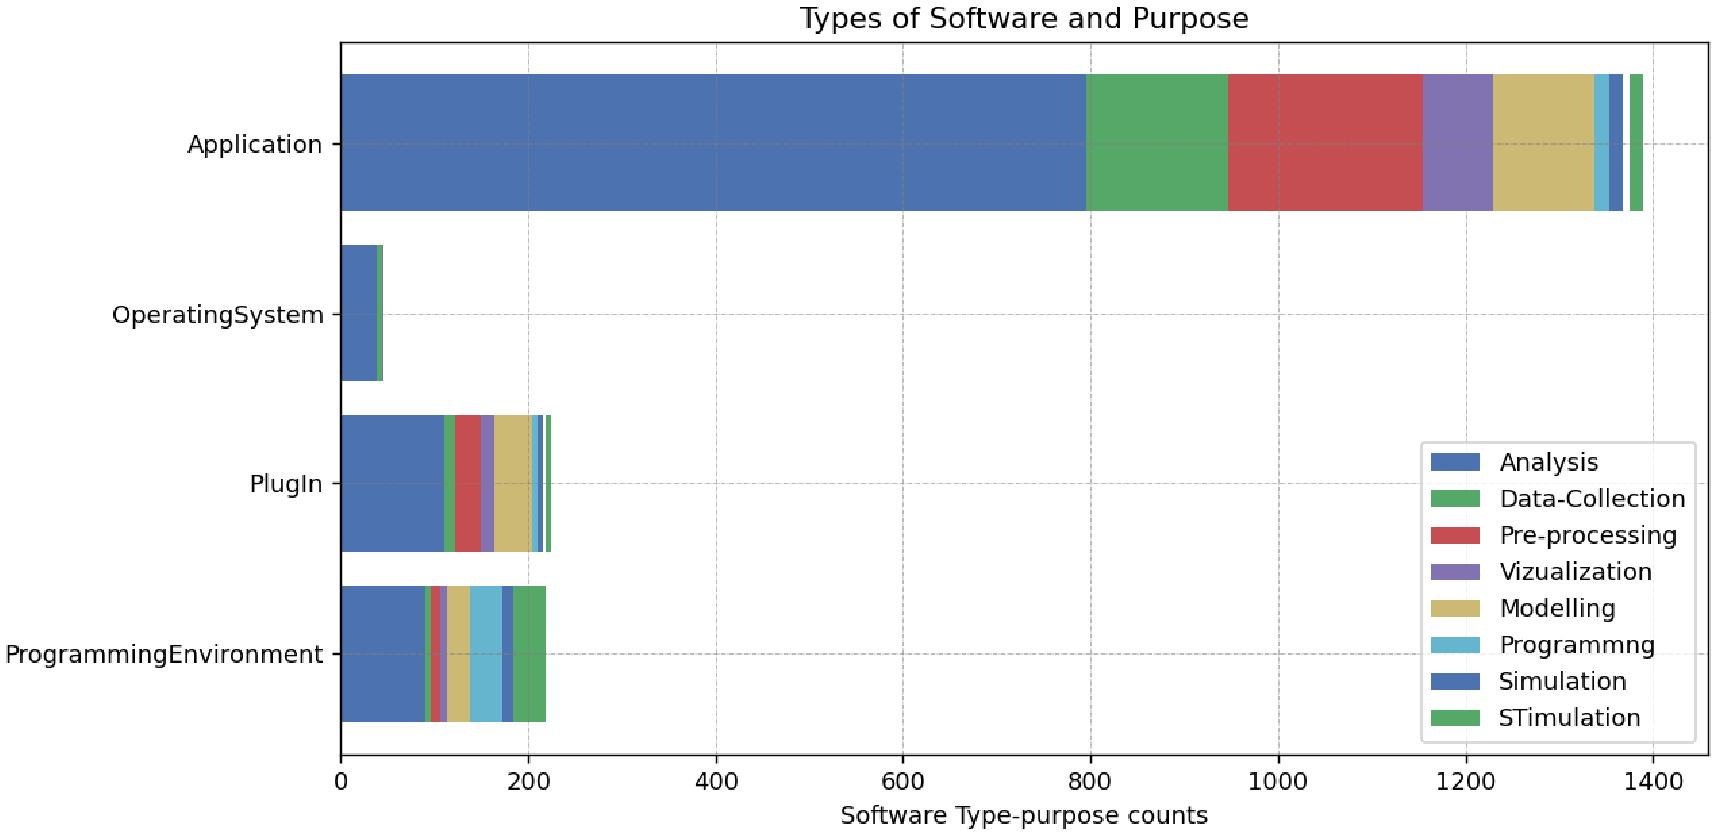
\includegraphics[width=1\textwidth]{4.graphics/figures/ch_4/analysisresults/6.Types of Software and Purpose stacked bar}
	\caption{Share of software usage purpose from each type of software in the \ac{SoMeSci} data set.}
	\label{fig:chapter03:setup}
\end{figure}

Lastly, the most interesting insight that is important for the automatic classification task was determining: ” for how many different purposes a given software have been used for ?”.  The analysis result reveals that from 657 unique software lists, a little over 3 out of 4 software have been used only for a single purpose. \\

Over all almost 98\% of software have been used for a purposes maximum of three. This indicates that most of the software have been used only for a specific purpose.  


\begin{figure}[h]
	
	\myfloatalign
	
	\subfloat{
		\label{fig:chapter03:subfloat:grafik1}
		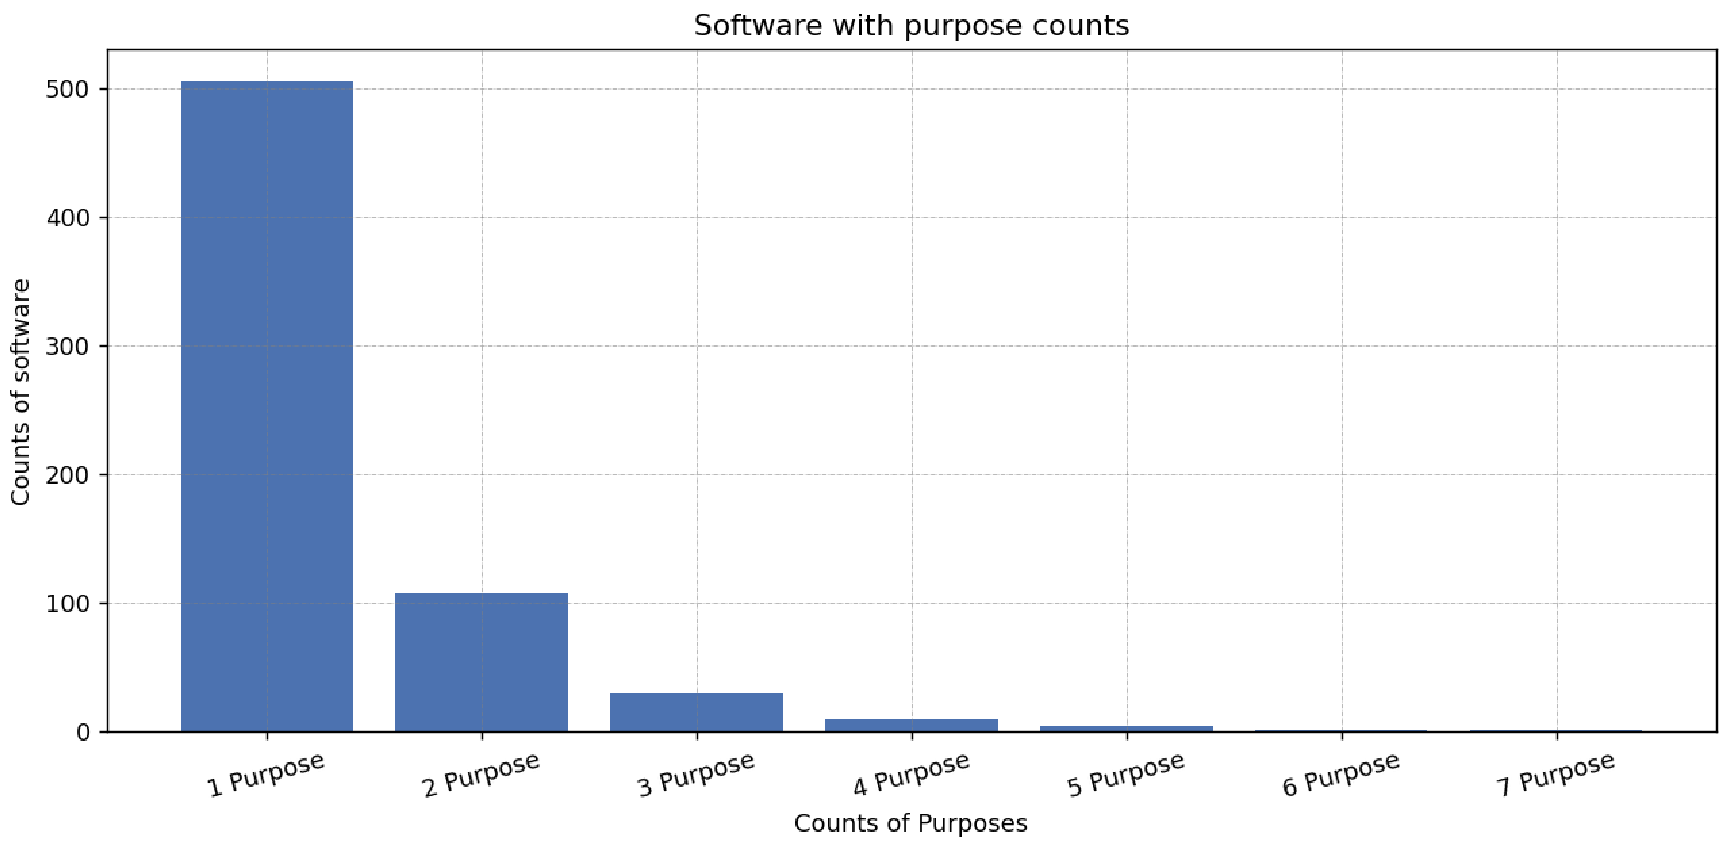
\includegraphics[width=1\linewidth]{4.graphics/figures/ch_4/analysisresults/7.counts of software purpose}
	} \\
	\subfloat{
		\label{fig:chapter03:subfloat:grafik4}
		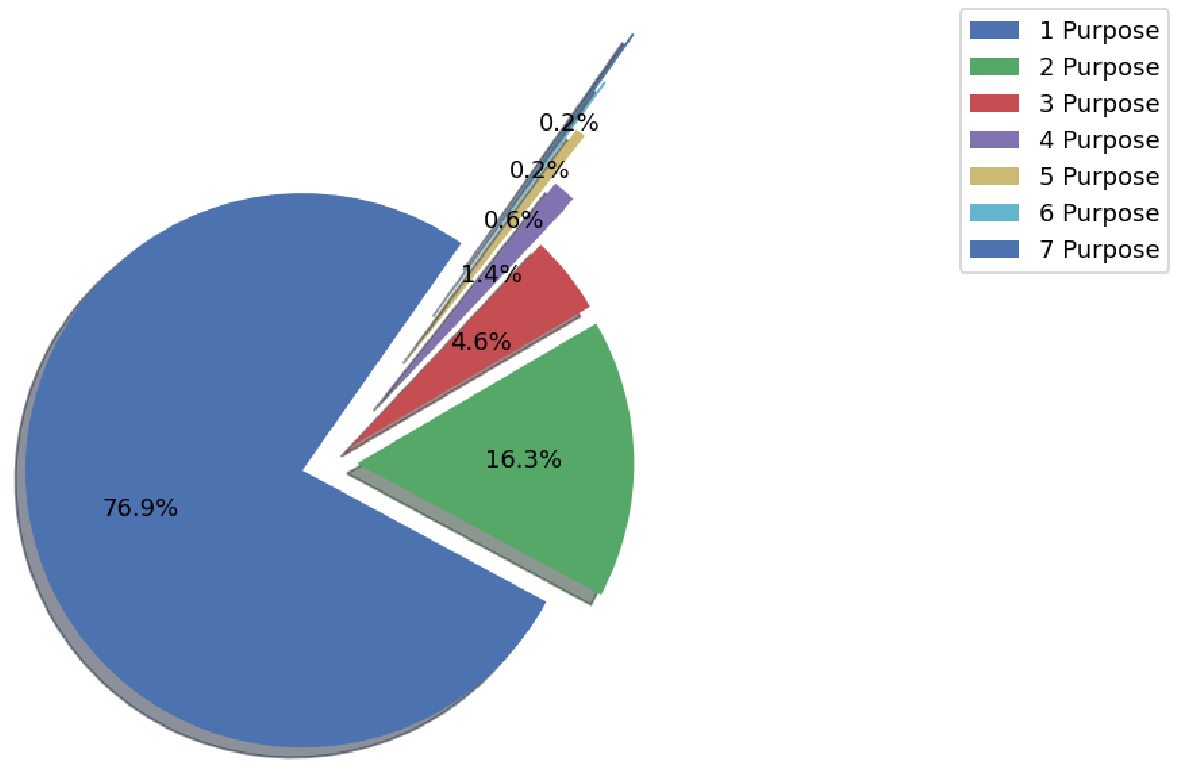
\includegraphics[width=.65\linewidth]{4.graphics/figures/ch_4/analysisresults/8.counts of software purpose pie}
	}\\
	\caption[Subfloat - Figure]{Merged software usage and purpose annotation \& its corresponding BIO representation.}
\end{figure}


